\section{Рабочий проект}
\subsection{Описание классов и функций}
\begin{lstlisting}[language=Python]
def open_add_window():  Открывает новое окно (Toplevel) для добавления информации о недвижимости в базу данных.

def add_realty(): Добавляет информацию об объекте недвижимости в базу данных. Эта функция определена внутри 

open_add_window() и имеет доступ к виджетам этого окна.

def open_salee_window(): открывает новое окно (Toplevel) для просмотра данных о продажах из таблицы sale базы данных.

def create_agreement(): создает договор купли-продажи на основе выбранной записи в списке продаж.

def open_view_window(): эта функция отвечает за создание и отображение окна просмотра объектов недвижимости. Она извлекает данные об объектах из базы данных и отображает их в окне с возможностью прокрутки.

def open_work_window(): эта функция создает окно для добавления информации о новом сотруднике.

def add_employee(): эта функция отвечает за получение данных о новом сотруднике из полей ввода, проверку (хотя бы минимальную) и добавление этой информации в таблицу employee в базе данных.


def open_worker_window(): эта функция отвечает за создание и отображение окна для просмотра списка сотрудников, хранящегося в базе данных.

def open_buy_window(): эта функция отвечает за создание окна, предназначенного для добавления информации о новом покупателе (или арендаторе). Она создает элементы интерфейса, необходимые для ввода данных о покупателе.

def add_client(): эта функция предназначена для добавления информации о новом клиенте (покупателе/арендаторе) в базу данных. Она собирает данные из полей ввода, выполняет минимальную проверку и добавляет запись в таблицу client.

def open_buyer_window(): эта функция открывает окно для просмотра списка клиентов (покупателей/арендаторов), извлекая данные из базы данных и отображая их.

def open_sell_window(): эта функция отвечает за создание окна, в котором пользователь может ввести данные о новом владельце (продавце/арендодателе) недвижимости.

def open_seller_window(): эта функция создает окно для просмотра списка владельцев (продавцов/арендодателей) недвижимости, извлекая данные из базы данных и отображая их в виде списка.

def open_sale_window(): эта функция отвечает за создание окна для ввода данных о новой продаже (заключении договора купли-продажи) и добавления этой информации в базу данных.

def add_sale(): Определяет функцию, которая будет вызываться при нажатии кнопки «Добавить». Эта функция собирает данные из полей ввода, проверяет их и добавляет новую запись в таблицу sale в базе данных.

def generate_sale_agreement(row): эта функция генерирует текст договора купли-продажи на основе данных, полученных из базы данных. Она принимает строку данных (row) в качестве аргумента и формирует текстовое представление договора, готовое к отображению или печати.

def open_salee_window(): эта функция отвечает за создание окна для просмотра информации о существующих договорах купли-продажи. Она извлекает данные о продажах из базы данных, отображает их в виде списка и предоставляет возможность сгенерировать текст договора для выбранной продажи.

def save_agreement(): эта функция позволяет сохранить сгенерированный текст договора (хранящийся в переменной agreement) в текстовый файл, выбранный пользователем с помощью диалогового окна сохранения файла.

def open_rent_window(): эта функция отвечает за создание окна, предназначенного для ввода информации о договоре аренды. 

def add_renta(): эта функция предназначена для добавления данных о новом договоре аренды в базу данных. Она собирает информацию из полей ввода в графическом интерфейсе, а затем вставляет эту информацию в таблицу renta. Также добавляет сообщение об успешном выполнении и закрывает окно.

def generate_rent_agreement(row): эта функция генерирует текст договора аренды на основе данных, полученных из строки базы данных. Функция формирует текст договора, который можно отобразить пользователю или сохранить в файл.

def open_rentt_window(): эта функция создает окно для просмотра договоров аренды. Она извлекает данные из базы данных и отображает их в виджете Listbox. Также предоставляет возможность сгенерировать договор аренды на основе выбранной записи.

save_agreement(): эта функция позволяет сохранить сгенерированный текст договора аренды (который хранится в переменной agreement) в текстовом файле. Пользователь может выбрать место и имя файла с помощью стандартного диалогового окна сохранения файла.
\end{lstlisting}  

\subsection{Тестирование разработанной программной системы}

Для работы пользователей с созданной базой данных было разработано десктопное приложение для ОС Windows. Для разработки приложения использовался язык программирования Python с фреймворком Qt, в состав которого входят библиотеки для разработки графического интерфейса и средства взаимодействия с базами данных.

Структура приложения показана на рисунках 4.13 – 4.30.

На рисунке \ref{главн_окно:image} представлено главное окно программы.

\begin{figure}[H]
\center{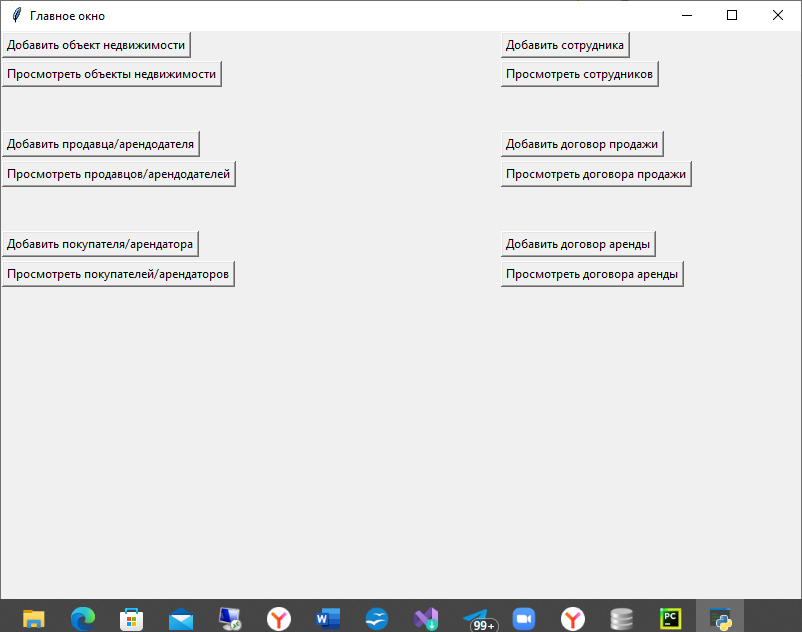
\includegraphics[width=0.8\linewidth]{главн_окно}}
\caption{Главное окно программы}
\label{главн_окно:image}
\end{figure}

На рисунке \ref{объект:image} представлено окно для добавления объектов недвижимости.

\begin{figure}[H]
	\center{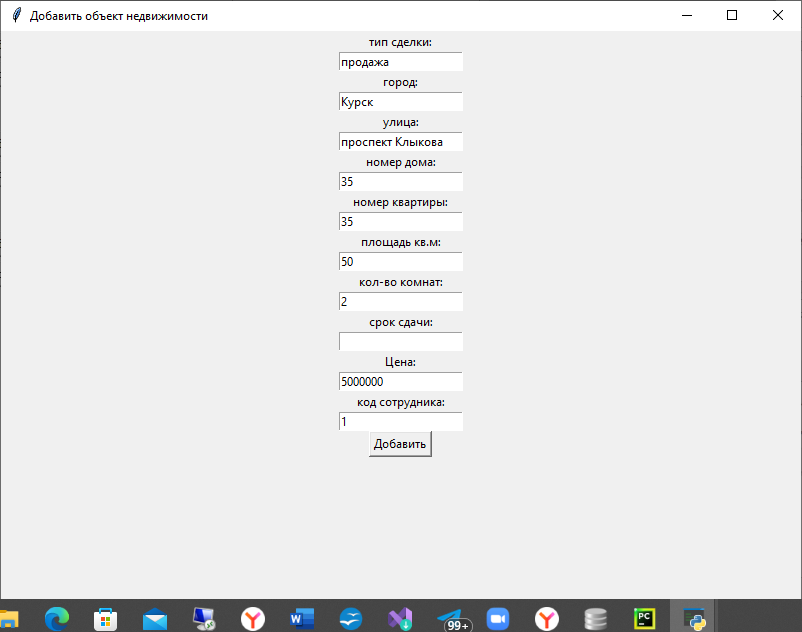
\includegraphics[width=0.8\linewidth]{объект}}
	\caption{Окно для добавления объектов недвижимости}
	\label{объект:image}
\end{figure}

На рисунке \ref{РОбъект:image} представлен результат добавления объекта недвижимости.

\begin{figure}[H]
	\center{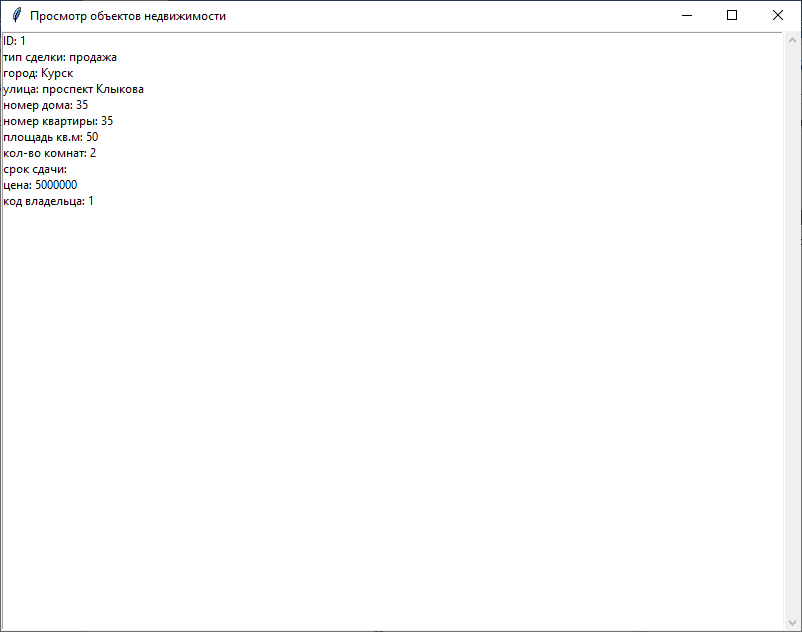
\includegraphics[width=0.8\linewidth]{РОбъект}}
	\caption{Результат добавления объекта недвижимости}
	\label{РОбъект:image}
\end{figure}

На рисунке \ref{номердома:image} представлена попытка ввести некорректные данные в поле номер дома.

\begin{figure}[H]
	\center{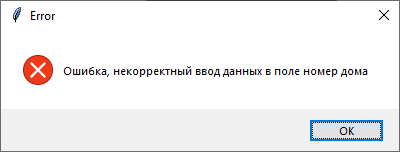
\includegraphics[width=0.4\linewidth]{номердома}}
	\caption{Попытка ввести некорректные данные в поле номер дома}
	\label{номердома:image}
\end{figure}

На рисунке \ref{невсеполя:image} представлена попытка добавить данные, не заполнив все поля.

\begin{figure}[H]
	\center{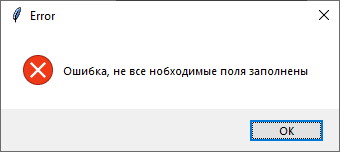
\includegraphics[width=0.4\linewidth]{невсеполя}}
	\caption{Попытка добавить данные, не заполнив все поля}
	\label{невсеполя:image}
\end{figure}\\

На рисунке \ref{продавец:image} представлено окно для добавления данных продавца/арендадателя.

\begin{figure}[H]
	\center{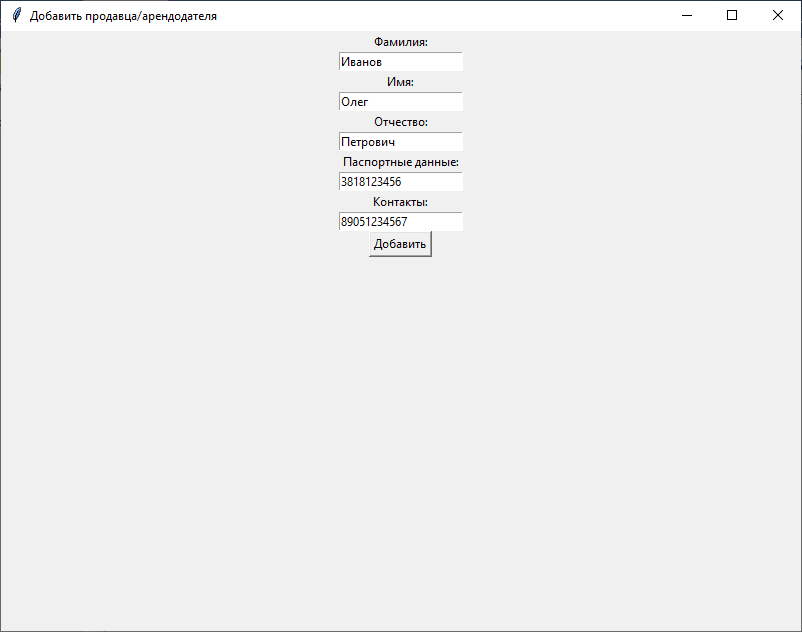
\includegraphics[width=0.8\linewidth]{продавец}}
	\caption{Окно для добавления данных продавца/арендадателя}
	\label{продавец:image}
\end{figure}

На рисунке \ref{РПродавец:image} представлен результат добавления данных продавца/арендадателя.

\begin{figure}[H]
	\center{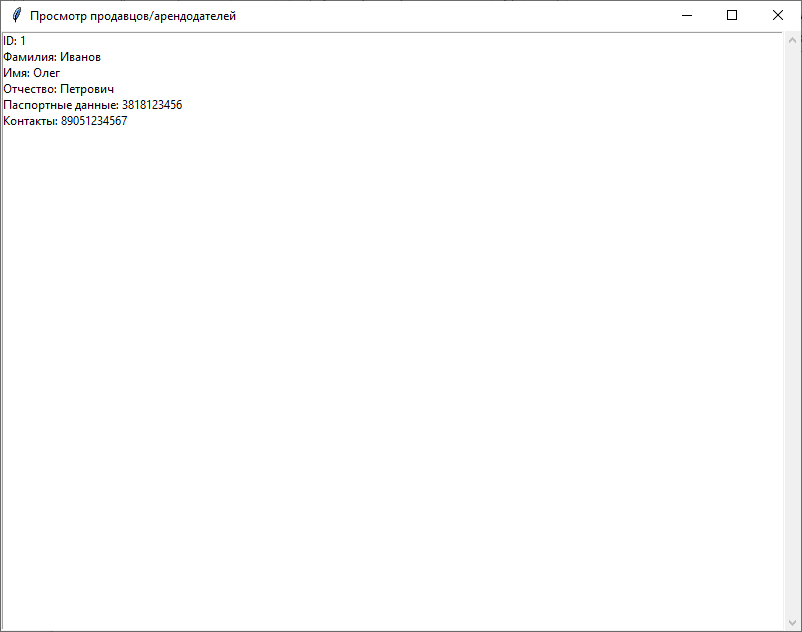
\includegraphics[width=0.8\linewidth]{РПродавец}}
	\caption{Результат добавления данных продавца/арендадателя}
	\label{РПродавец:image}
\end{figure}

На рисунке \ref{покупатель:image} представлено окно для добавления данных покупателя/арендатора.

\begin{figure}[H]
	\center{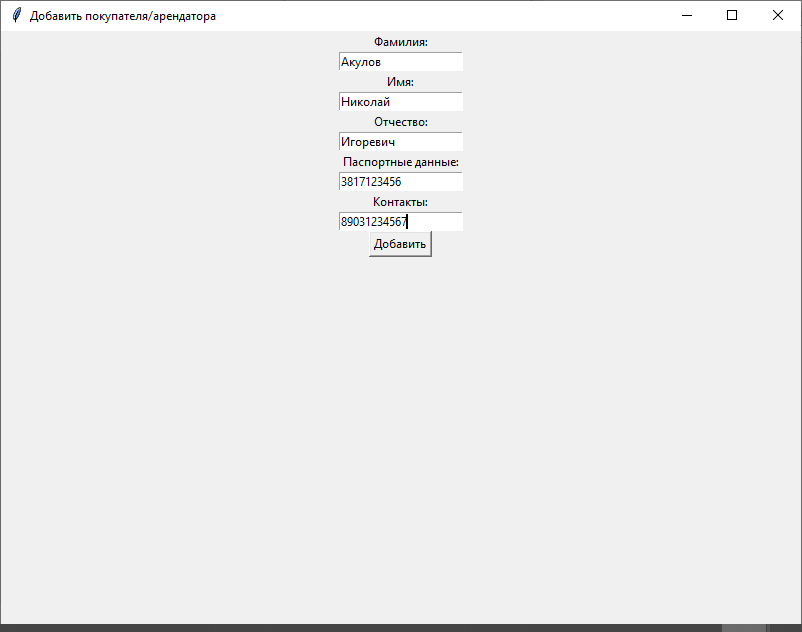
\includegraphics[width=0.8\linewidth]{Покупатель}}
	\caption{Окно для добавления данных покупателя/арендатора}
	\label{покупатель:image}
\end{figure}

На рисунке \ref{рпокпатель:image} представлен результат добавления данных покупателя/арендатора.

\begin{figure}[H]
	\center{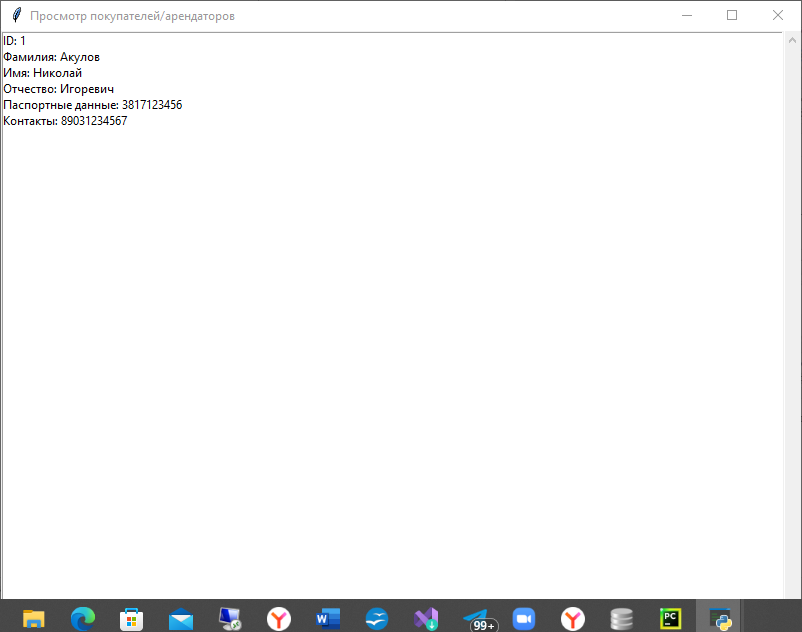
\includegraphics[width=0.8\linewidth]{РПокупатель}}
	\caption{Результат добавления данных покупателя/арендатора}
	\label{рпокупатель:image}
\end{figure}

На рисунке \ref{сотрудник:image} представлено окно для добавления данных сотрудника.

\begin{figure}[H]
	\center{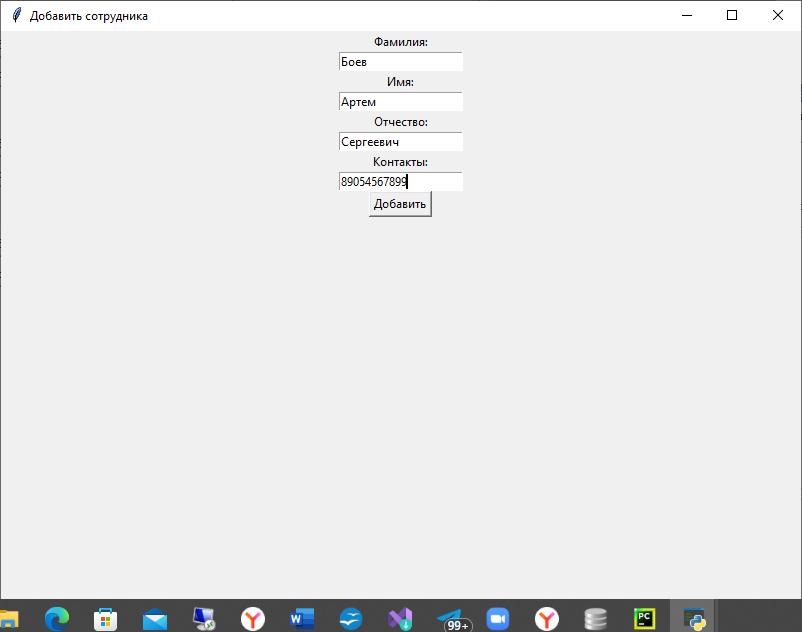
\includegraphics[width=0.8\linewidth]{Сотрудник}}
	\caption{Окно для добавления данных сотрудника}
	\label{сотрудник:image}
\end{figure}

На рисунке \ref{рсотрудник:image} представлен результат добавления данных сотрудника.

\begin{figure}[H]
	\center{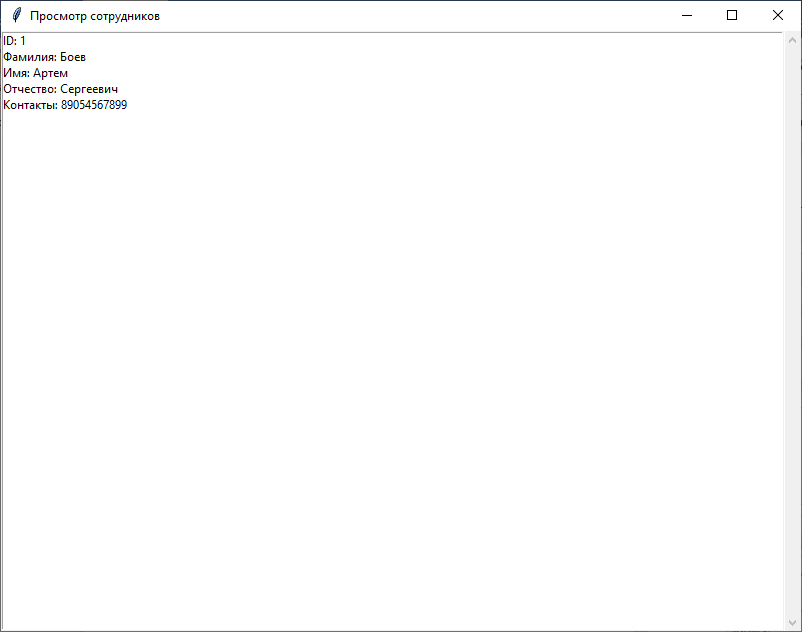
\includegraphics[width=0.8\linewidth]{РСотрудник}}
	\caption{Результат добавления данных сотрудника}
	\label{рсотрудник:image}
\end{figure}

На рисунке \ref{продажи:image} представлено окно для добавления данных договора продажи.

\begin{figure}[H]
	\center{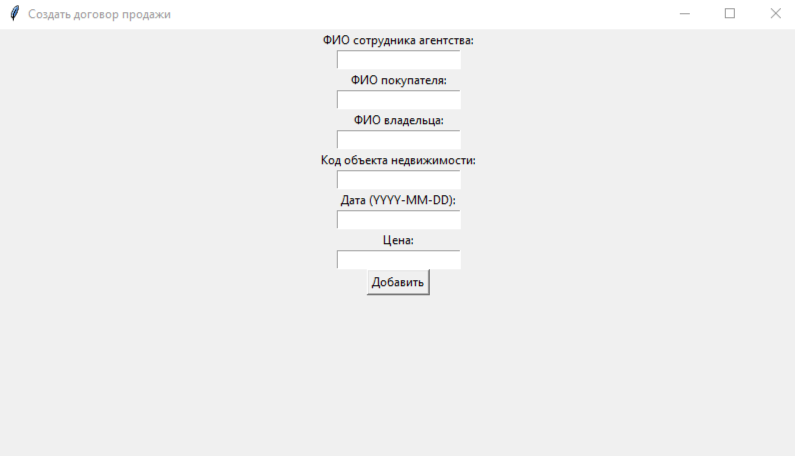
\includegraphics[width=0.8\linewidth]{Продажи}}
	\caption{Окно для добавления данных договора продажи}
	\label{продажи:image}
\end{figure}

На рисунке \ref{рпродажи:image} представлены данные для создания договора продажи.

\begin{figure}[H]
	\center{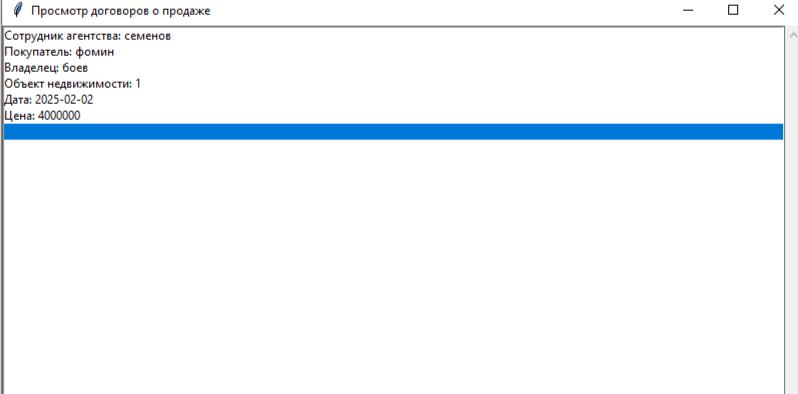
\includegraphics[width=0.8\linewidth]{РПродажи}}
	\caption{Данные для создания договора продажи}
	\label{рпродажи:image}
\end{figure}

На рисунке \ref{договорП:image} представлен созданный договор продажи.

\begin{figure}[H]
	\center{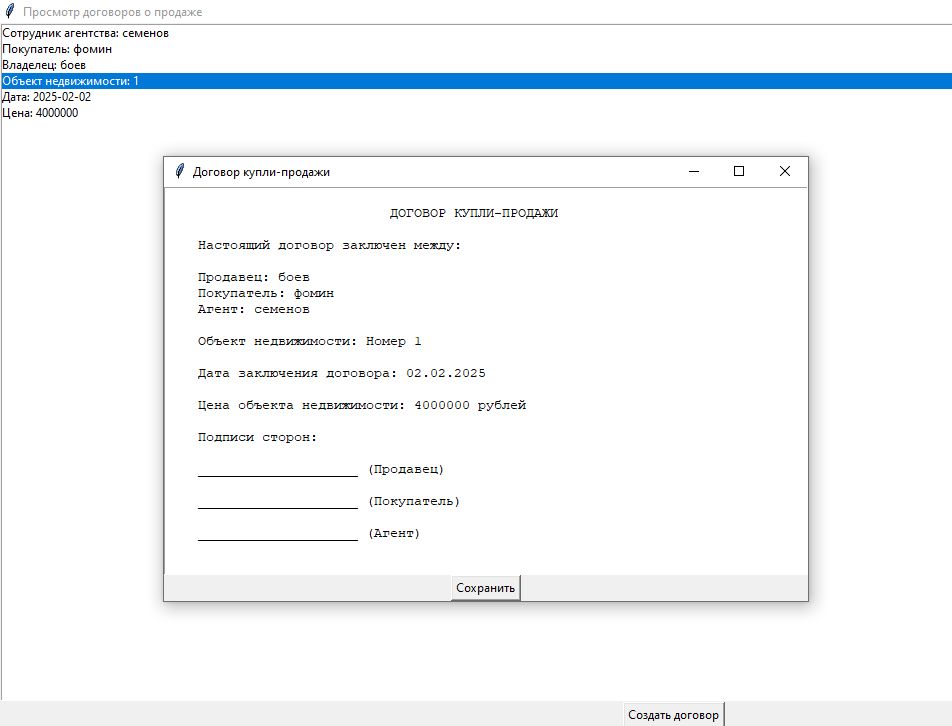
\includegraphics[width=0.8\linewidth]{ДоговорП}}
	\caption{Созданный договор продажи}
	\label{договорП:image}
\end{figure}

На рисунке \ref{аренда:image} представлено окно для добавления данных договора аренды.

\begin{figure}[H]
	\center{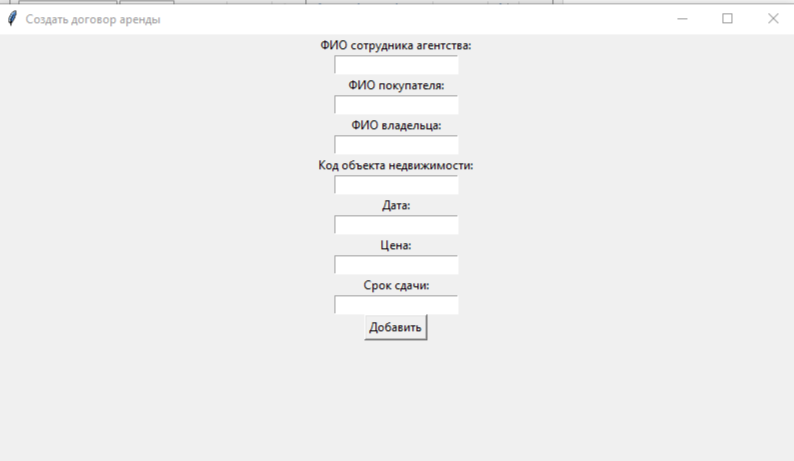
\includegraphics[width=0.8\linewidth]{Аренда}}
	\caption{Окно для добавления данных договора аренды}
	\label{аренда:image}
\end{figure}

На рисунке \ref{раренда:image} представлены данные для создания договора аренды.

\begin{figure}[H]
	\center{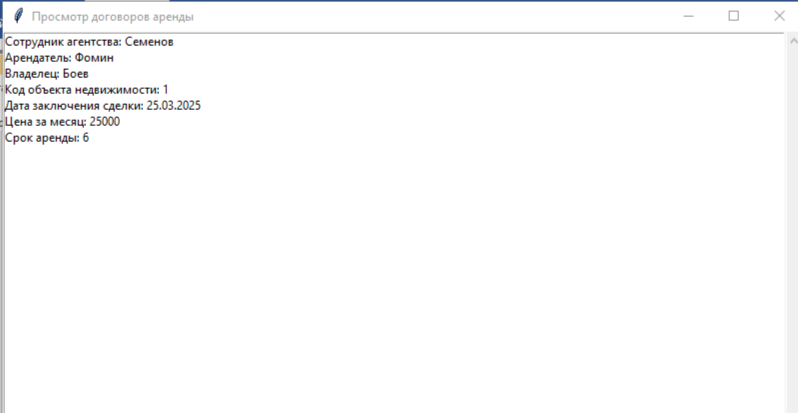
\includegraphics[width=0.8\linewidth]{РАренда}}
	\caption{Данные для создания договора аренды}
	\label{раренда:image}
\end{figure}

На рисунке \ref{даренда:image} представлен созданный договор аренды.

\begin{figure}[H]
	\center{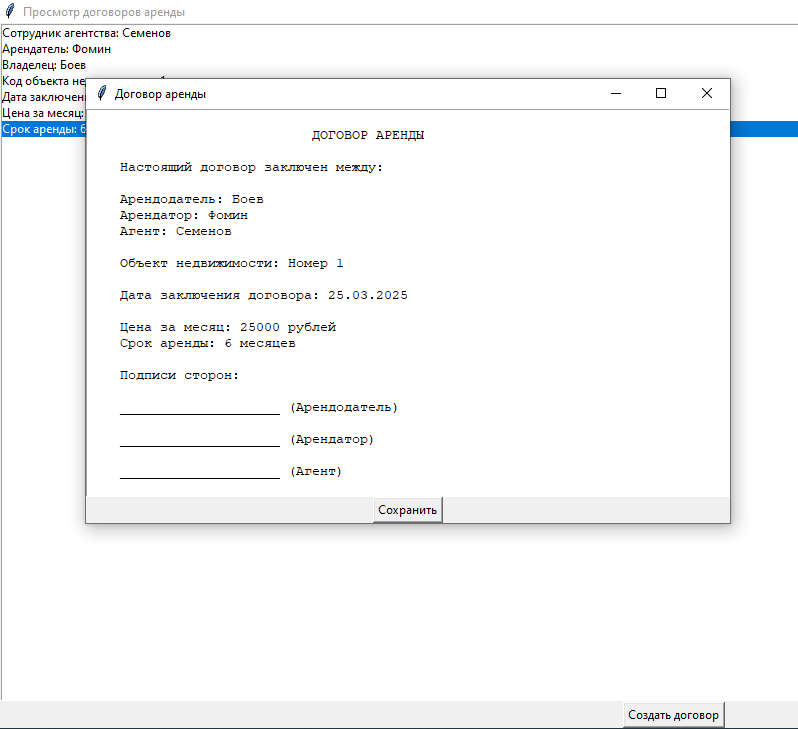
\includegraphics[width=0.8\linewidth]{ДоговорА}}
	\caption{Созданный договор аренды}
	\label{даренда:image}
\end{figure}\\

На рисунке \ref{успех:image} представлено уведомление об успешной загрузке данных в базу данных.

\begin{figure}[H]
	\center{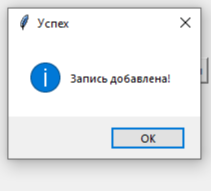
\includegraphics[width=0.4\linewidth]{успех}}
	\caption{Уведомление об успешной загрузке данных в базу данных}
	\label{успех:image}
\end{figure}

На рисунке \ref{пустой:image} представлена попытка создать пустой договор.

\begin{figure}[H]
	\center{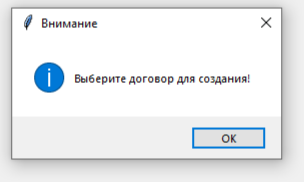
\includegraphics[width=0.4\linewidth]{пустойД}}
	\caption{Попытка создать пустой договор}
	\label{пустой:image}
\end{figure}